\begin{flushleft}
    \section{Analysis}
        \subsection{Statment Of Problem}
        \large
        \bk
        Maps, as you would think of them today, have been arround since 6\textsuperscript{th} century BC and since then have been in constant use by people in their day to day lives. 
        The more modern version of maps, for example Google maps or Bing maps have only been around since the late 1990's. The problem that I am going to be solving is map pathfinding.
        Currently not all roads and paths are logged and entered into a searchable format. The only way some people have to navigate terrain is through the use of old style paper maps.
        The problem with paper maps is that they are not easily, at a glance, used to find a path from point to point. As well as this sometimes are not easy to comprehend just by looking 
        at them with various terrain features. \\
        
        \bk
        \begin{figure}[h]
            \centering
            \subfloat[\centering Map without labeles on roads]{{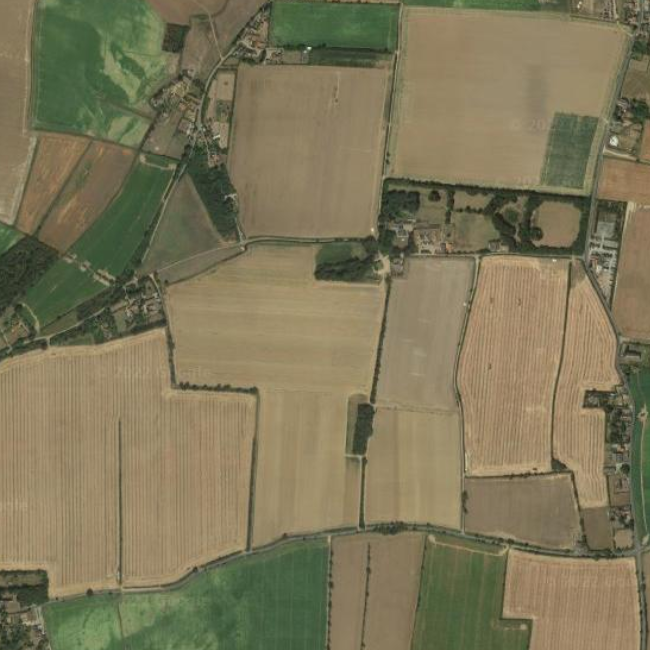
\includegraphics[width=6cm]{images/unlabeledMap.png}}}
            \qquad
            \subfloat[\centering Map with labeles on roads]{{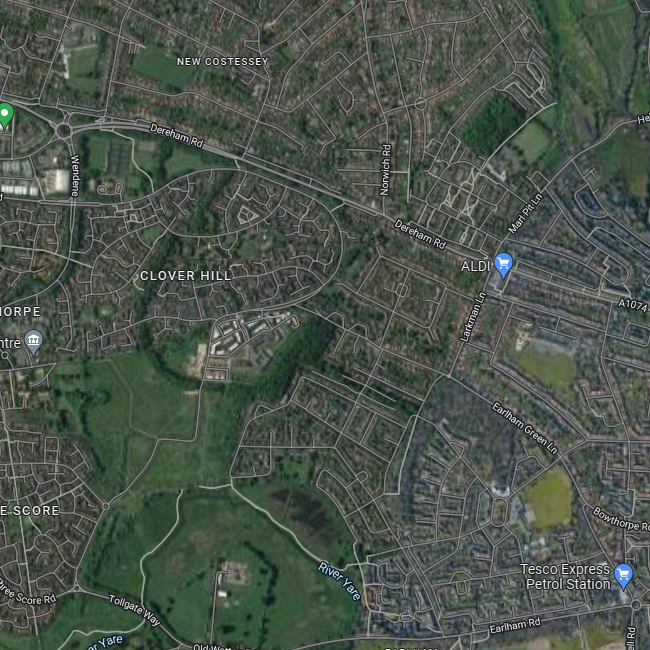
\includegraphics[width=6cm]{images/labeledMap.png}}}
            \caption*{Examples of maps with and without lables taken from Google Maps\textsuperscript{\textcopyright}}
        \end{figure}
        \bk

        This can cause issues for people who live out in areas which have not been mapped. This is because they cannot create easy to follow routes with the click of a button. Therefor, 
        causing people who live in rural areas to waste time getting used to the routes they have to take to go anywhere. Overall, the problem I am going to be creating a solution for is 
        how people are unable to easily go from point to point at the click of a button and be easily able to, at a glance, interpret the map without prior expeirence. \\

        \subsection{Background}
        \bk
        \lipsum[2]
        \subsection{End User}
            \subsubsection{Initial Interview}
            \lipsum[2]
        \bk

\end{flushleft}